% Draft report generated from the committed results pack (reports/tables, reports/figures, reports/RESULTS_REGISTER.md).
% Every number below is transcribed from a table named in its caption; none was computed in this file.
% Author name: not set (config.yaml author = TO_CONFIRM). Add it on the title page only after it is confirmed.
% Items marked [VERIFY] must be checked against the original source before submission.
\documentclass[12pt]{report}
\usepackage[a4paper,margin=1in]{geometry}
\usepackage{graphicx,booktabs,float,caption,hyperref,setspace,amsmath}
\usepackage[backend=bibtex,style=numeric]{biblatex}
\addbibresource{ref.bib}
\graphicspath{{figures/}}
\onehalfspacing
\newcommand{\unexpl}{\emph{not explained by measured cost drivers}}

\begin{document}

\begin{titlepage}
\centering
{\Large \textbf{Bangladesh Food Price Watch}}\\[1.2em]
{\large Forecasting Dhaka daily retail food prices from external drivers\\and flagging rises that measured costs do not explain}\\[3em]
Project report (draft)\\[1em]
Author: [to be confirmed]\\
Supervisor: [to be confirmed]\\
Department / University: [to be confirmed]\\[2em]
\today
\end{titlepage}

\chapter*{Abstract}
Food prices in Bangladesh rise sharply from time to time, and it is hard to tell how much of a rise is explained by costs that can be measured. This project builds a daily price panel of 63 essential items from the Trading Corporation of Bangladesh (TCB) Dhaka retail reports (17 May 2021 to 24 October 2026, 1{,}412 report days) and joins it to external drivers: world commodity prices, Brent oil, the exchange rate, diesel prices, import volumes, weather, fishing bans and policy events. Every driver is dated by the day it was available, and the 2022 reporting gap is never filled.

We ask whether classical models, LightGBM and drivers improve forecasts over ``tomorrow equals today'' (RQ1, RQ2), whether forecast intervals raise alerts on documented price shocks at a fixed false-alarm rate (RQ3), and how much of each flagged rise the drivers explain (RQ4). The test period (January 2025 to October 2026) was scored once, after pre-registration.

No model beat the naive forecast in the all-items summary at any horizon. LightGBM with the core features had a geometric-mean relative MAE of 1.001, 1.015, 1.028 and 1.085 at horizons 1, 7, 14 and 30 report days, and no driver group was significantly better than the core model on any mapped item after Holm correction. The pre-registered alert rule detected 7 of 12 documented shock episodes (0.583), but placebo event dates detected 0.479 (95\% range 0.25--0.67), so the detection rate is not distinguishable from chance with this few events. For most flagged rises the measured drivers explained a small share, and the remainder is reported as \unexpl. These results are a careful negative finding, not evidence about the cause of any price rise.

\tableofcontents
\listoffigures
\listoftables

\chapter{Introduction}
\section{Background}
Staple food prices matter directly for household welfare in Bangladesh. Rice, edible oil, sugar, onion, eggs and lentils absorb a large share of spending, and sharp rises attract public attention and policy responses. Official monitoring of retail prices exists, but there is no open, English, machine-readable daily record of the TCB reports, and published forecasting work on Bangladeshi retail prices covers few items and uses price history alone.

\section{Motivation}
Two questions follow. First, do outside cost factors help predict prices beyond the price's own recent value? Second, when a price rises unusually fast, how much of the rise do those factors account for? The second question must be answered carefully: a rise that measured costs do not explain may have many causes (an unmeasured cost, a local supply shock, a quality change). The project therefore reports such rises only as \unexpl.

\section{Research questions}
\begin{description}
\item[RQ1] Does any model beat ``tomorrow equals today'' at horizons of 1, 7, 14 and 30 report days, and for which item groups?
\item[RQ2] Do external drivers, added one group at a time to a core model and compared with a placebo assignment, improve forecasts, and for which items?
\item[RQ3] Do forecast-interval alerts flag documented price shocks, and at what false-alarm rate?
\item[RQ4] How much of a flagged rise is explained by measured cost drivers, and how much is not?
\end{description}
A fifth question, locating a rise nationally or in single markets with WFP monthly market prices, was not answered because that stage was not built (Section~\ref{sec:limits}).

\section{Organisation}
Chapter 2 reviews related work, Chapter 3 describes data and methods, Chapter 4 reports results, and Chapter 5 concludes with limitations.

\chapter{Literature Review}
\textit{Status: starter review written from search summaries. Items marked [VERIFY] were not read in full (see docs/LITERATURE\_REVIEW.md).}

\section{Forecasting retail food prices}
A 2026 benchmark on the AgriPriceBD dataset, five commodities over July 2020 to June 2025, compared Naive persistence, SARIMA, Prophet, BiLSTM, Transformer variants and Informer using price history only \cite{agripricebd}. It found no single model best everywhere; naive persistence was best for four of the five commodities, and Prophet failed on step-like prices. Other studies report gains from tree ensembles over a random walk for food price indices in other countries, but often against weak baselines and at index or monthly level [VERIFY]. Evidence that drivers add value for Bangladeshi daily retail prices, item by item, was not found.

\section{External drivers and pass-through}
Studies of Bangladesh report partial pass-through of world food price shocks to domestic prices, with an estimate near 46\% in one error-correction study [VERIFY], and strong influence of imported onion prices on local onion prices \cite{onionnardl}. Pass-through is partial and lagged, which motivates dating each driver by its true availability date and testing driver groups only on the items they plausibly affect.

\section{Evaluation methods}
Forecast accuracy is reported as relative MAE against the naive forecast and as MASE, which scales errors by the in-sample naive error \cite{hk2006}. Forecasts are compared with the Diebold--Mariano test \cite{dm1995} with the Harvey--Leybourne--Newbold small-sample correction \cite{hln1997}, and p-values within a driver group are adjusted with the Holm procedure. Foundation models such as Chronos-2 accept covariates \cite{chronos2}; they were not implemented in this project.

\chapter{Methodology and Data}
\section{Research design}
The design is a pre-registered forecasting experiment. All tuning uses calendar 2024. The test period, January 2025 to October 2026, is scored once per stage after the pre-registration file is committed (Table~\ref{tab:drivers} lists the data used). Time is measured in TCB report days, not calendar days.

\section{Core price data}
The TCB panel holds 63 item--unit series, 1{,}412 report days and 76{,}440 rows. Only 24 reports exist between 12 March and 31 December 2022; that period is used as history only and no price is filled across it. Nine series with short histories (for example green chilli and cucumber, from February 2026) are scored separately, leaving 54 long-history series. Two typographical errors were corrected and the Palm Olein 2~L row of 18 April 2025 is flagged but not changed without approval.

\section{External drivers}
\begin{table}[H]\centering\small
\caption{Driver slots and availability dating (source: reports/tables/T3.csv).}\label{tab:drivers}
\begin{tabular}{p{3.0cm}p{5.6cm}p{2.6cm}p{2.2cm}}
\toprule
Slot & Source & Frequency & Available \\ \midrule
G1 own world price & IMF: soybean oil, palm oil, wheat, Thai rice, milk & monthly & month end + 40 d \\
G2 own Brent & FRED Brent oil & daily & as of date \\
G3 export measure & India onion duty, MEP, ban (reconstructed) & event & start date \\
G4 fishing ban & hilsa, jatka and marine bans & event & announced dates \\
G5 weather & three features chosen on 2024 & daily & date + 5 d \\
E1 exchange rate & BDT/USD, spliced series & daily & as of date \\
E2 diesel & administered price & event & effective date \\
E3 imports & Comtrade mirror data by HS code & monthly & month start + 208 d \\
E4 events & exporter measures, disruptions, floods, duty cuts & event & event dates \\
\bottomrule
\end{tabular}
\end{table}
Slots G1--G5 enter the forecasting models; E1--E5 are used only in the explanation step. A driver with no mapped value stays empty with a \texttt{has\_} flag, never zero. Import data are stamped as available 208 days after the start of the month; an earlier 75-day stamp was a bug and the leakage test fails if it is used.

\section{Models and evaluation}
Seven classical models were re-run (Naive, SeasonalNaive, WindowAverage, random walk with drift, AutoARIMA, AutoETS, AutoTheta) over 87 forecast origins, together with LightGBM. The core LightGBM model uses price history and calendar features; driver groups are added one at a time in the pre-registered order on their mapped items only. Each driver is compared with the same group assigned to unmapped items (placebo, fixed seed). Metrics are the geometric mean of relative MAE against naive, MASE and win rate; tests are Diebold--Mariano with the Harvey--Leybourne--Newbold correction and Holm adjustment at $\alpha=0.05$.

\section{Alerts and explanation}
The expected price is a real-time LightGBM forecast at horizon 7. The upper bound is a trailing conformal quantile of past residuals (window 120 report days), and an alert needs 3 of the last 5 report days above the bound. The operating level (0.975) was fixed from 2024 non-event false-alarm rates before events were scored. For explanation, three nested models (M0 price and calendar, M1 plus forecasting drivers, M2 plus explanation drivers) split a realised rise into shares, and the remainder is reported as \unexpl.

\section{Baseline reproduction}
The earlier classical baseline was re-run. Naive matches exactly and AutoETS is within 0.010 at every horizon. AutoTheta (horizon 1, +0.273), AutoARIMA (horizons 1 to 30, +0.027 to +0.063), WindowAverage (horizon 1, +0.025) and SeasonalNaive (horizon 1, +0.021) differ by more than the 0.02 tolerance. The original settings were never recorded, so the likely causes (gap handling in the training input and automatic model selection) are hypotheses, and nothing was tuned to close the gap (docs/REPRO\_EXPLAINED\_2026-11-11.md).

\chapter{Results}
\section{RQ1: benchmark against naive}
\begin{table}[H]\centering\small
\caption{Geometric-mean relative MAE vs.\ naive, all long-history items (source: reports/tables/T4.csv, stratum ALL). Values above 1 are worse than naive.}\label{tab:rq1}
\begin{tabular}{lrrrr}
\toprule
Model & h=1 & h=7 & h=14 & h=30 \\ \midrule
Naive & 1.000 & 1.000 & 1.000 & 1.000 \\
LGBM core & 1.001 & 1.015 & 1.028 & 1.085 \\
LGBM core + forecasting drivers (M1) & 1.004 & 1.019 & 1.020 & 1.066 \\
AutoETS & 1.178 & 1.046 & 1.039 & 1.033 \\
AutoARIMA & 1.493 & 1.228 & 1.186 & 1.158 \\
AutoTheta & 1.574 & 1.191 & 1.180 & 1.158 \\
Random walk with drift & 1.269 & 1.307 & 1.296 & 1.275 \\
WindowAverage & 3.271 & 1.326 & 1.145 & 1.060 \\
SeasonalNaive & 5.157 & 1.000 & 1.000 & 1.108 \\
\bottomrule
\end{tabular}
\end{table}
No model has a summary below 1.000 at any horizon. The closest are LightGBM at short horizons and AutoETS at longer ones, and none is significantly better than naive. This agrees with the earlier five-item benchmark \cite{agripricebd}. Figure~\ref{fig:rq1} shows the pattern by horizon.
\begin{figure}[H]\centering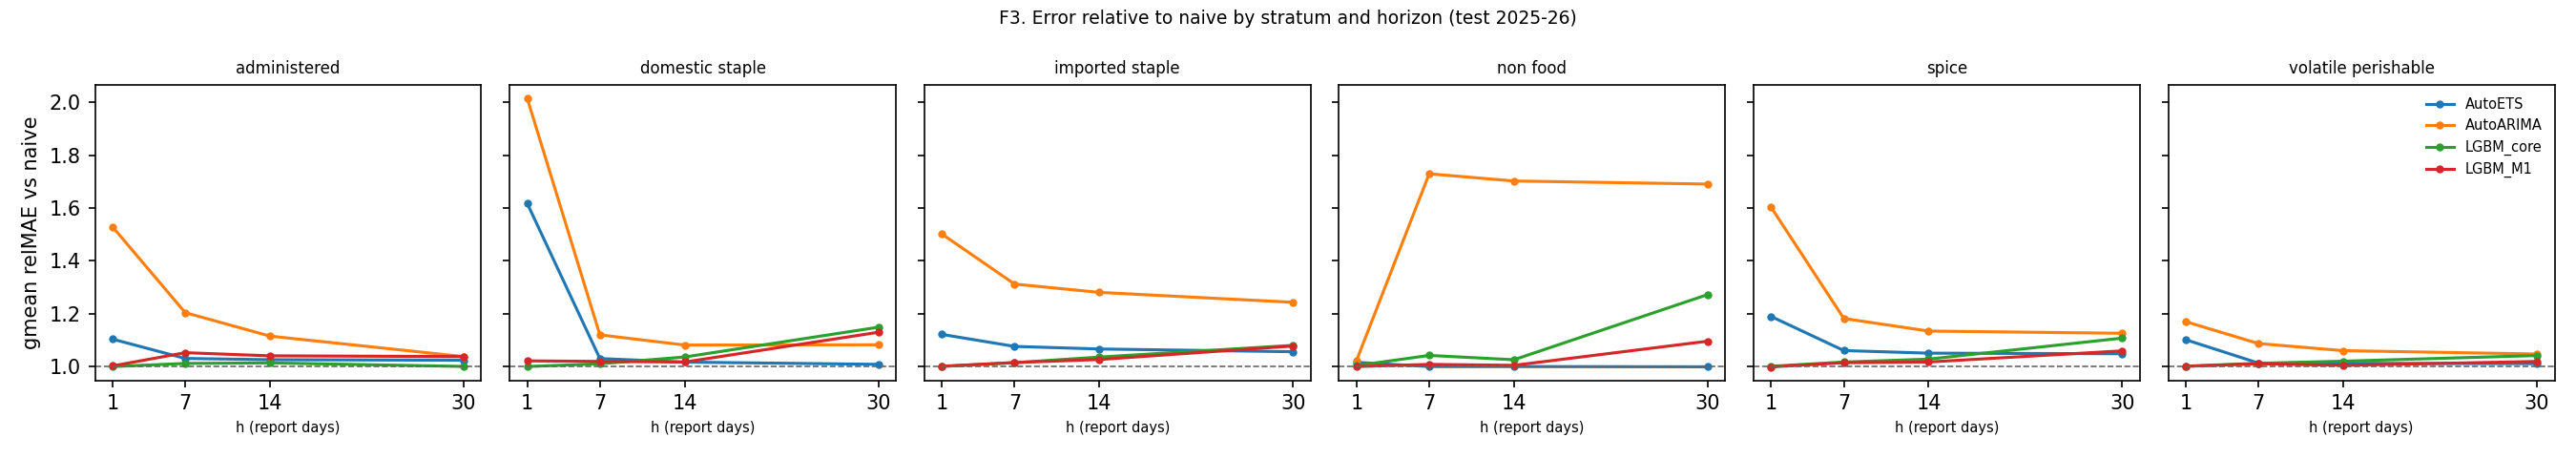
\includegraphics[width=0.85\textwidth]{F3_relmae_by_horizon.png}\caption{Relative MAE by horizon (reports/figures/F3).}\label{fig:rq1}\end{figure}

\section{RQ2: value of drivers}
Table~\ref{tab:rq2} summarises the change in relative MAE when a driver group is added to the core model (positive means worse), for matched items and for the placebo assignment.
\begin{table}[H]\centering\small
\caption{Mean change in relative MAE, matched vs.\ placebo, selected rows (source: reports/tables/T5b.csv). No row has a matched item significantly better than core after Holm correction.}\label{tab:rq2}
\begin{tabular}{lrrrr}
\toprule
Group & h & Matched items & Matched change & Placebo change \\ \midrule
G1 world price & 7 & 17 & +0.0301 & +0.0030 \\
G1 world price & 30 & 17 & +0.0266 & +0.0089 \\
G2 Brent & 30 & 5 & +0.0068 & +0.0237 \\
G3 export measure & 14 & 2 & +0.0216 & $-$0.0112 \\
G5 weather & 14 & 4 & $-$0.0366 & +0.0156 \\
G5 weather & 30 & 4 & $-$0.0610 & +0.0572 \\
\bottomrule
\end{tabular}
\end{table}
World prices (G1) made forecasts slightly worse at horizons 7 to 30, with a matched-minus-placebo gap whose interval at horizon 7 excludes zero on the worse side. The only favourable pattern is weather (G5) at horizon 30 on four items (matched $-0.061$, placebo $+0.057$), but no item is significant after Holm correction and the number of items is small, so it is exploratory. G4 (fishing ban) has a single item and cannot be tested. Figure~\ref{fig:rq2} shows the comparison.
\begin{figure}[H]\centering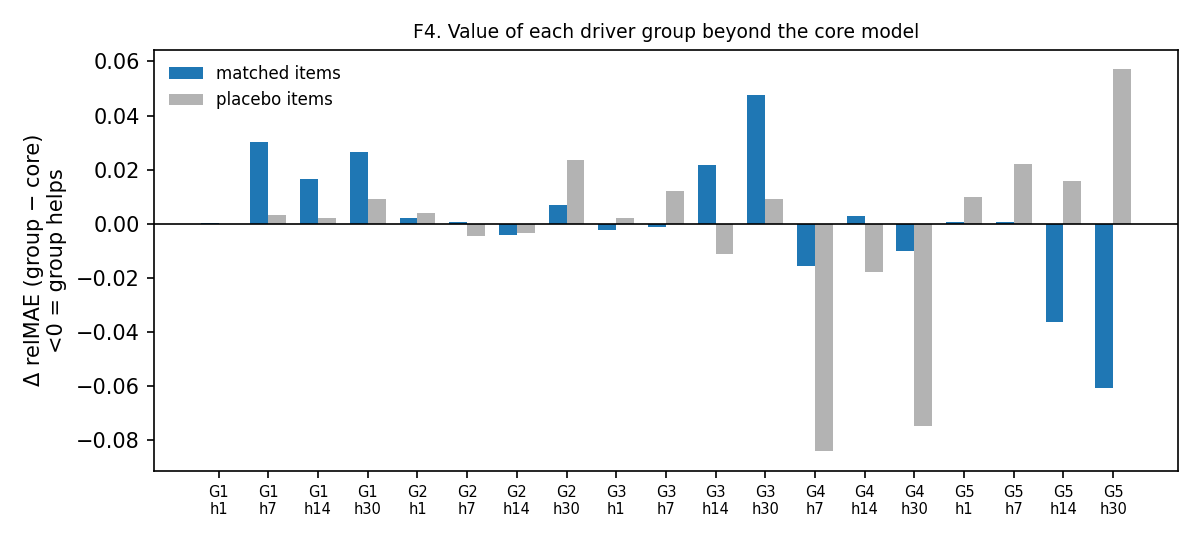
\includegraphics[width=0.85\textwidth]{F4_driver_value.png}\caption{Driver value, matched vs.\ placebo (reports/figures/F4).}\label{fig:rq2}\end{figure}

\section{RQ3: alerts}
The pre-registered rule has an upper 95\% bound coverage of 0.921 against a nominal 0.95, and the Kupiec test rejects correct coverage on non-event periods (Table~\ref{tab:cov}, stratum ALL, source reports/tables/T6.csv).
\begin{table}[H]\centering\small
\caption{Alert rules (source: reports/tables/T8.csv, stratum ALL). Recall is the share of the 12 in-window events detected; false alarms are per item-year.}\label{tab:alerts}
\begin{tabular}{lrrr}
\toprule
Rule & False alarms & Recall (12 events) & Clean-test recall \\ \midrule
Conformal 0.975, 3 of 5 (pre-registered) & 1.828 & 0.583 & 1.0 \\
Robust z$\ge$1 & 3.023 & 0.667 & 1.0 \\
Robust z$\ge$2 & 2.111 & 0.500 & 1.0 \\
Robust z$\ge$3 & 1.532 & 0.500 & 1.0 \\
ALPS-style z$\ge$1 & 0.562 & 0.500 & 0.0 \\
ALPS-style z$\ge$2 & 0.346 & 0.333 & 0.0 \\
IFPA-style $\ge$1 & 0.189 & 0.167 & 0.0 \\
IFPA-style $\ge$0.5 & 0.323 & 0.500 & 0.0 \\
\bottomrule
\end{tabular}
\end{table}
\begin{table}[H]\centering\small
\caption{Interval coverage, all items (source: reports/tables/T6.csv).}\label{tab:cov}
\begin{tabular}{lrrr}
\toprule
Stratum & Upper 95\% coverage & 90\% coverage & Kupiec p (non-event) \\ \midrule
ALL & 0.921 & 0.854 & $<0.001$ \\
\bottomrule
\end{tabular}
\end{table}
The pre-registered rule detected 7 of the 12 documented episodes: BD-S12, S13, S14, S15, S16, S21 and S22. Only one episode (BD-S22, July 2026) lies in the clean 2025--26 test; the others fall in periods used to fix the threshold, so detection there is not an independent test. Placebo event dates, with the same items and window lengths, were detected at 0.479 (95\% range 0.25--0.67; $p=0.285$). With this few events the rule is not distinguishable from chance.
\begin{figure}[H]\centering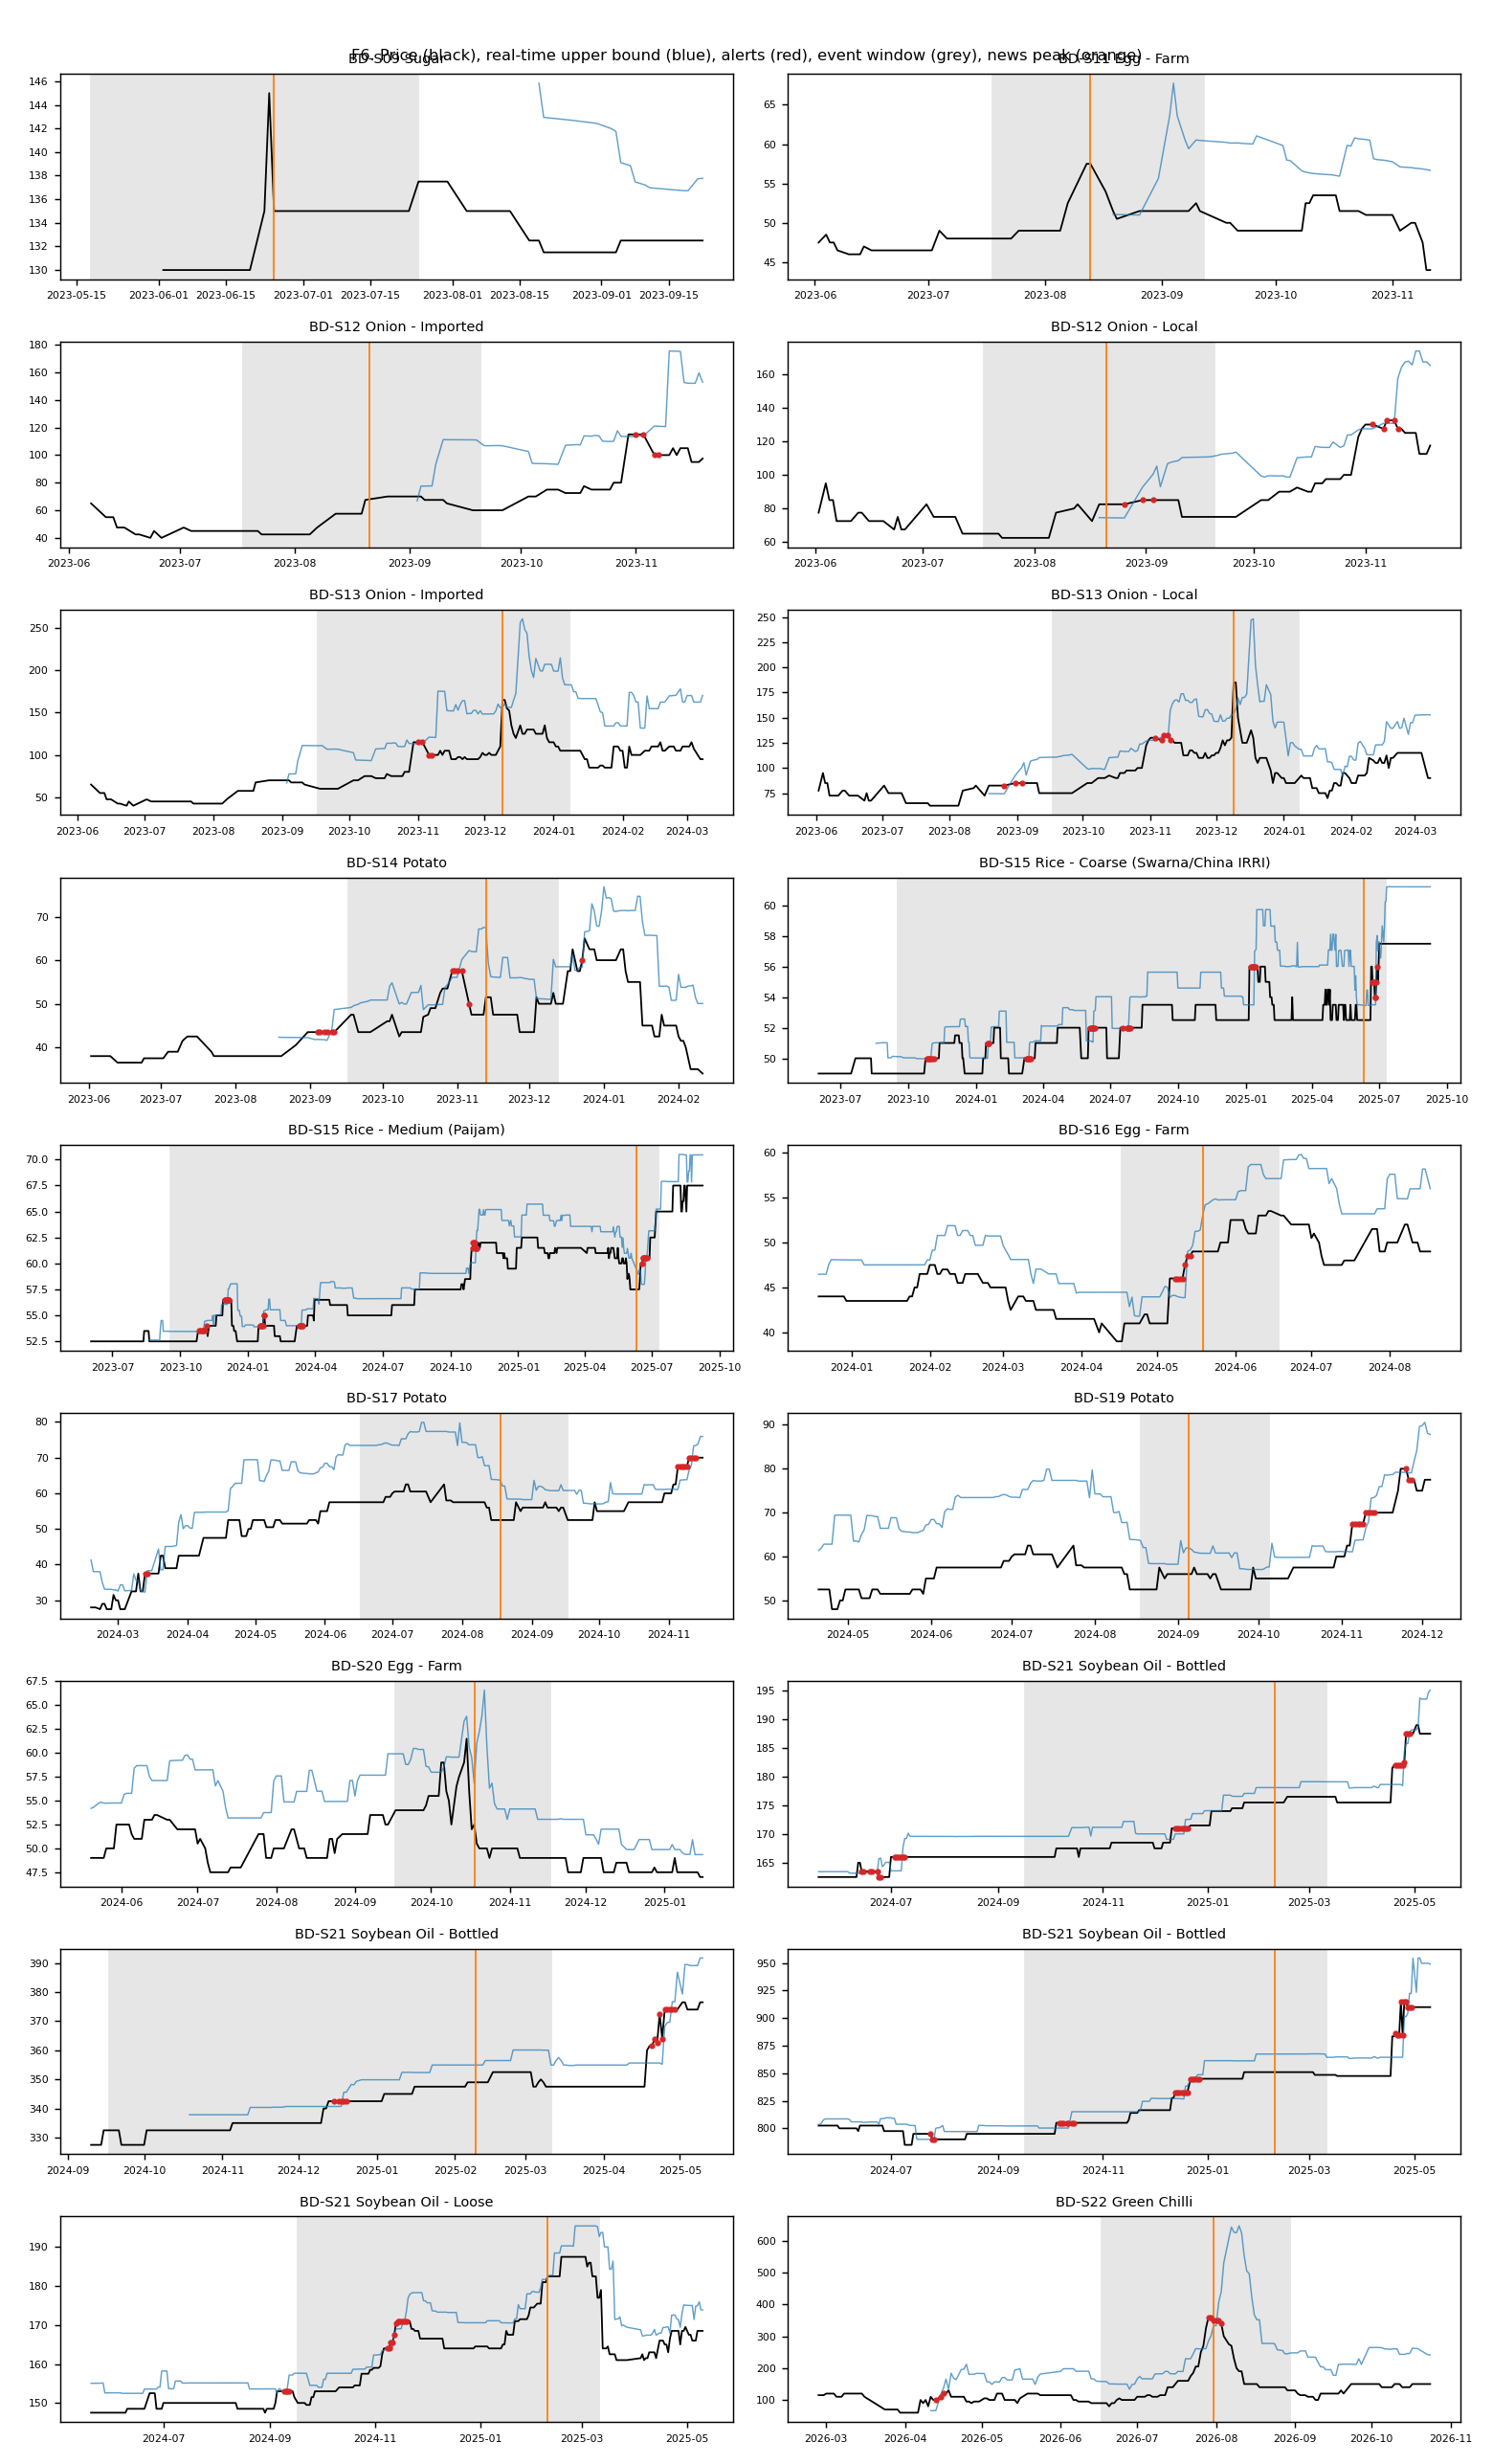
\includegraphics[width=0.85\textwidth]{F6_alert_timelines.png}\caption{Alert timelines for documented episodes (reports/figures/F6).}\label{fig:alerts}\end{figure}

\section{RQ4: explained and unexplained shares}
For the episodes with a realised rise, the measured drivers explained a small share of the rise in most cases (Table~\ref{tab:rq4}, source reports/tables/T9.csv); the remainder is \unexpl.
\begin{table}[H]\centering\small
\caption{Share of the realised rise not explained by measured cost drivers, selected episodes (source: reports/tables/T9.csv).}\label{tab:rq4}
\begin{tabular}{llrr}
\toprule
Episode & Item & Realised rise (\%) & Share not explained \\ \midrule
BD-S12 & Onion, imported & 35.3 & 0.97 \\
BD-S13 & Onion, imported & 66.7 & 0.74 \\
BD-S13 & Onion, local & 70.0 & 0.65 \\
BD-S21 & Soybean oil, 1~L & 5.7 & 0.83 \\
BD-S21 & Soybean oil, loose & 14.7 & 0.73 \\
\bottomrule
\end{tabular}
\end{table}
Two episodes (BD-S17 potato, BD-S20 eggs) show no rise over the window. For the long rice episode (BD-S15) the decomposition shares fall outside 0--1 because the explanation step offsets the other components, so they are not read as proportions. The event studies (reports/tables/T10.csv) find no abnormal change that is distinguishable from placebo dates for the verified India onion export ban of 8 December 2023 (7-day mean abnormal change 8.4\%, one-sided $p=0.124$) or for the BDT/USD jump of 10 May 2024 ($p$ between 0.107 and 0.226). The September 2023 price caps were not studied because no dated, sourced event was available.
\begin{figure}[H]\centering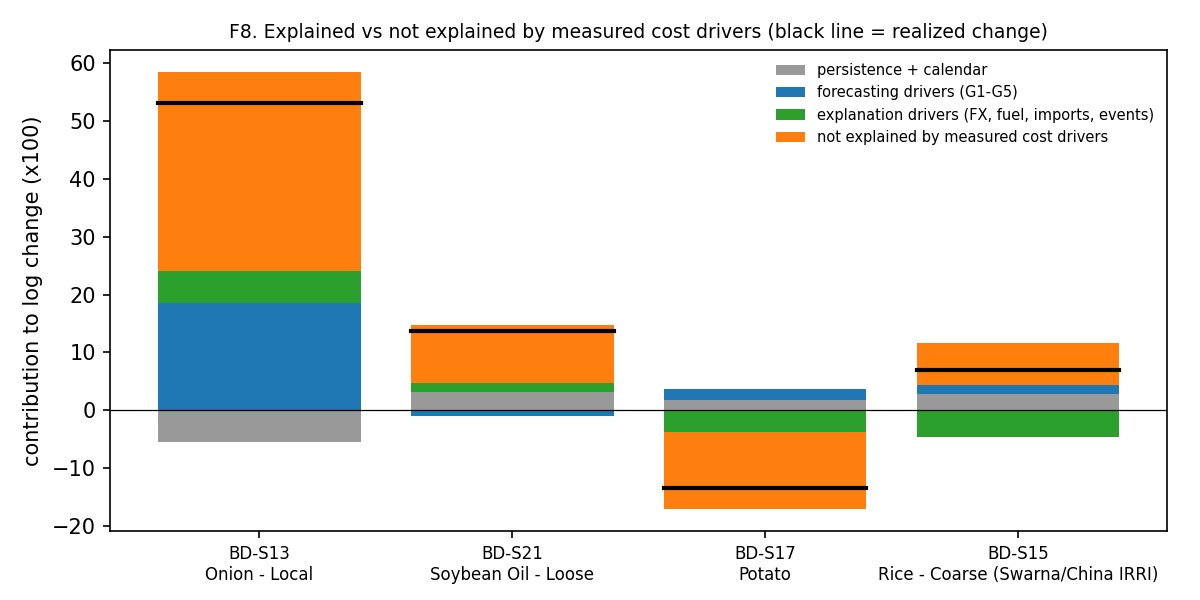
\includegraphics[width=0.85\textwidth]{F8_decomposition.png}\caption{Decomposition of realised rises (reports/figures/F8).}\label{fig:rq4}\end{figure}

\section{Robustness}
Replacing the expanding window with a sliding 500-report-day window, or removing the 2021 ginger candidates from the targets, does not change the RQ1 conclusion (LightGBM core stays between 1.000 and 1.134 against naive; reports/tables/T11.csv). Excluding events tied to reconstructed exporter dates gives a detection rate of 0.545; the alternative alert rules give 0.500 to 0.667. A weekly aggregation check, Min/Max targets and RQ5 robustness were not run.

\chapter{Conclusion and Limitations}
\section{Conclusion}
On TCB daily retail prices, nothing beat the naive forecast in the all-items summary, adding external drivers did not improve forecasts on any mapped item after correction for multiple testing, and the pre-registered alerts detected 7 of 12 documented episodes, a rate that placebo dates also reach. For most flagged rises the measured drivers account for a small share, which the report labels \unexpl. A negative result is itself informative: for short-horizon retail prices, persistence is a strong benchmark and the measured external drivers used here do not beat it.

\section{Limitations}\label{sec:limits}
\begin{itemize}
\item The audit (S02) was not done because the original TCB Excel files were not supplied, so the transcription error rate is unknown.
\item The WFP intake and locate stages (S03, S08) were not built, so RQ5 and the cross-checks with WFP, AgriPriceBD, the Pink Sheet and the OHLC dataset were not done.
\item Chronos-2 and other foundation models were not implemented.
\item The classical baseline reproduction differs from the earlier file for several models (Section 3.6); the cause is unconfirmed.
\item Only 12 shock episodes fall in the data, 11 of them in periods used to set the threshold; the clean test contains one.
\item India's exporter dates are partly reconstructed from news reports, and the 2022 reporting gap hides the 2022 fuel and edible-oil episodes.
\item TCB publishes no reuse terms; a no-objection should be requested before releasing the data.
\item An independent review (S99) has not been run.
\end{itemize}

\section{Future work}
Run the audit with the original files, add the WFP stages to test whether rises are national or local, test a foundation model with covariates under a new pre-registration, and extend the explanation step with measured transport and wage costs.

\printbibliography[heading=bibintoc,title={References}]
\end{document}
